%--------------------------------------------------------------------------------------------------------------------------------%
% Code for "Appendix C: Understanding how population structure affects pathogen richness in a mechanistic model of bat populations"
% Appendix for Chapter 3 of thesis "The role of population structure and size in determining bat pathogen richness"
% by Tim CD Lucas
%
% NB The file is numbered Appendix2 as Chapter 3 was previously Chapter 2 in the thesis.
%
%---------------------------------------------------------------------------------------------------------------------------------%


















% --------------------------------------------------------------------------- %
% Invading pathogen plots
% --------------------------------------------------------------------------- %




\begin{knitrout}\footnotesize
\definecolor{shadecolor}{rgb}{0.969, 0.969, 0.969}\color{fgcolor}\begin{figure}[t]

{\centering 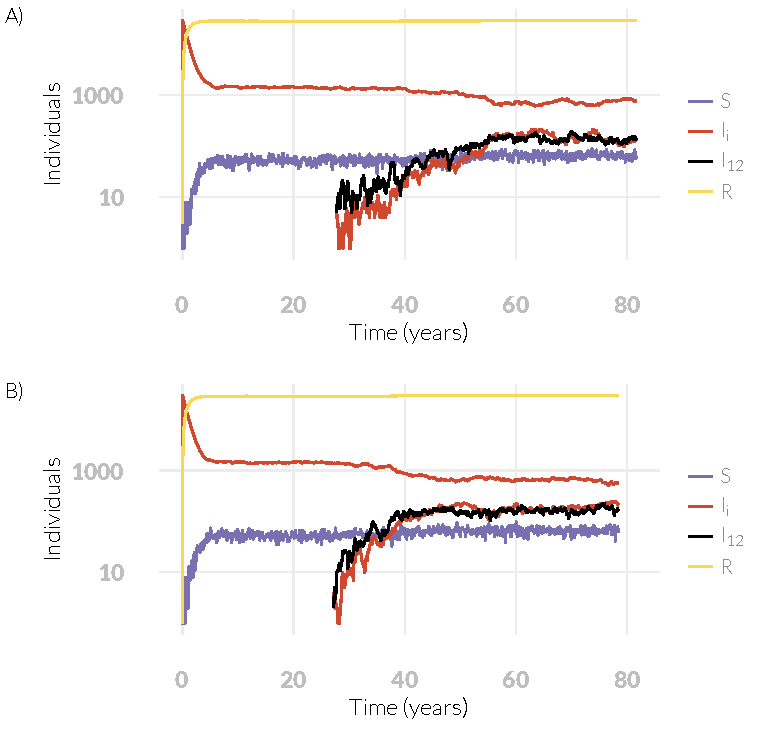
\includegraphics[width=\textwidth]{figure/A-plotsInvade-1} 

}

\caption[
Examples of simulated SIR dynamics with successfull invasions
]{
Two examples (A and B) of a successful invasion plotted on a logged $y$-axis.
The lines are coloured such that blue represents susceptibles, brown represents individuals infected with one pathogen (the two seperate brown lines are Pathogen 1 and 2), black represents co-infected individuals and yellow represents recovered and immune individuals.
Pathogen 2 is seeded after \SI{300000} events (approximately 30 years).
Simulations are run on a fully-connected network.
Parameter values are: dispersal rate = 0.1, transmission rate = 0.2.
All other parameters are as stated in Table~\ref{t:params}.
}\label{fig:plotsInvade}
\end{figure}


\end{knitrout}



% --------------------------------------------------------------------------- %
% No invasion plots
% --------------------------------------------------------------------------- %







\begin{knitrout}\footnotesize
\definecolor{shadecolor}{rgb}{0.969, 0.969, 0.969}\color{fgcolor}\begin{figure}[t]

{\centering 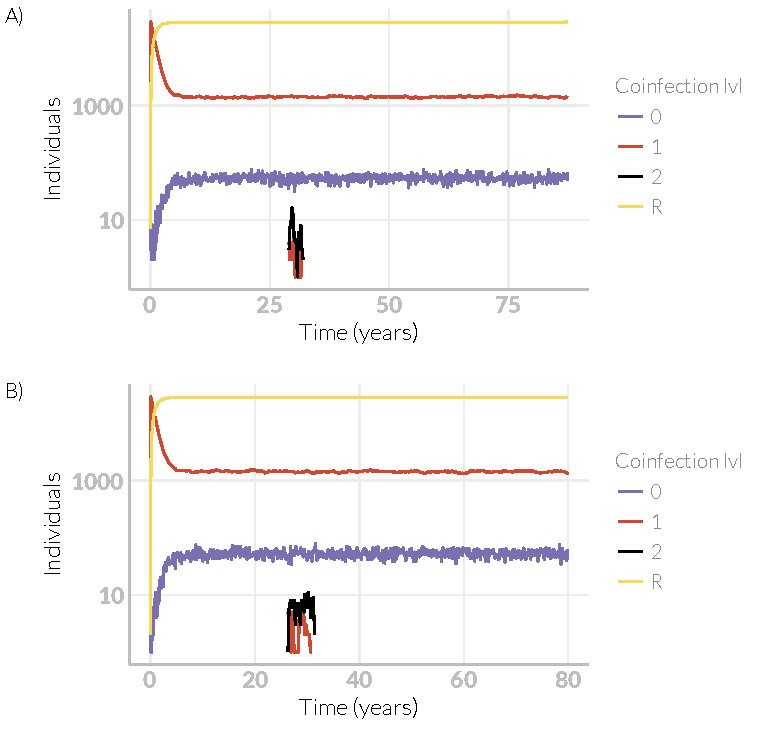
\includegraphics[width=\textwidth]{figure/A-plotsNoInvade-1} 

}

\caption[
Examples of simulated SIR dynamics with unsuccessfull invasions
]{
Two examples (A and B) of an unsuccessful invasion plotted on a logged $y$-axis.
The lines are coloured such that blue represents susceptibles, brown represents individuals infected with one pathogen (the two separate brown lines are Pathogen 1 and 2), black represents co-infected individuals and yellow represents recovered and immune individuals.
Pathogen 2 is seeded after \SI{300000} events (approximately 30 years).
It can be seen that after seeding Pathogen 2, there is a very short period before extinction as opposed to a long fade out of disease.
Simulations are run on a fully-connected network.
Parameter values are: dispersal rate = 0.1, transmission rate = 0.2.
All other parameters are as stated in Table~\ref{t:params}.
}\label{fig:plotsNoInvade1}
\end{figure}

\begin{figure}[t]

{\centering 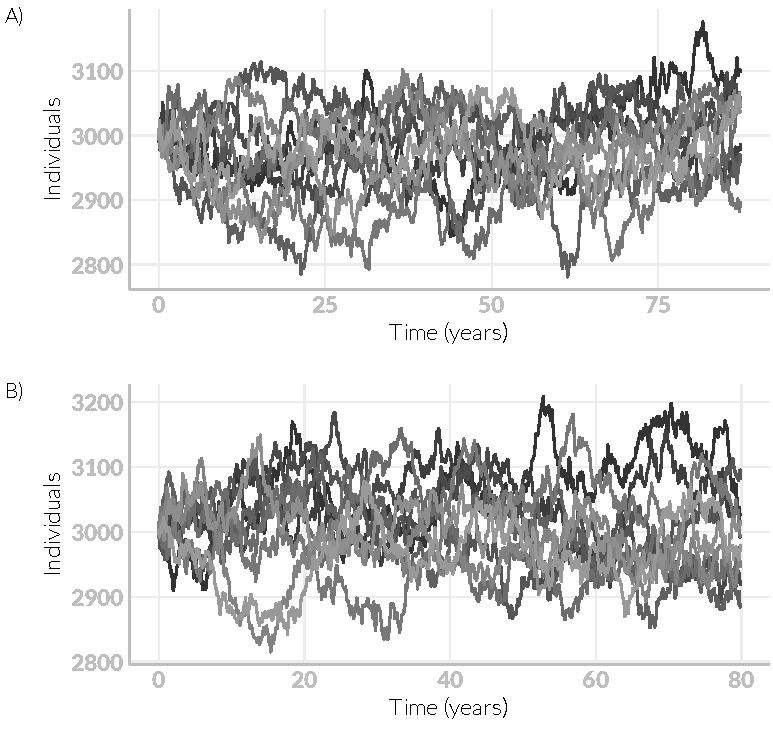
\includegraphics[width=0.8\textwidth]{figure/A-plotsNoInvade-2} 

}

\caption[
Examples of colony size dynamics
]{
Two examples (A and B) of the change in colony sizes throughout a simulation (note the truncated $y$-axis).
The size of each colony changes as a random walk.
However, given the length of the simulations, there is little risk of colonies going extinct or becoming very large.
Birth and death rate are equal and set to 0.05, giving a generation time of 20 years.
The metapopulation network is fully-connected and the dispersal rate is 0.1 per year.
The starting colony size is \SI{3000}.
}\label{fig:plotsNoInvade2}
\end{figure}


\end{knitrout}














% ------------------------------------------------------------------ %
% Topology Sims
% ------------------------------------------------------------------ %

















% ------------------------------------------------ %
% Raw data tables
% ------------------------------------------------ %








































\clearpage
% latex table generated in R 3.3.1 by xtable 1.8-2 package
% Mon Jul 25 00:04:16 2016
\begin{table}[ht]
\centering
\caption[
Raw data for dispersal simulations
  ]{
Raw data for dispersal simulations.
The relevant parameters are shown along with the number of invasions and the number of simulations.
$\beta$ is the transmission rate.
} 
\label{B-disp}
\begingroup\small
\begin{tabular}{@{}rrrr@{}}
  \toprule
$\beta$ & Dispersal & Invasions & Sims \\ 
  \midrule
0.1 & 0.000 & 0 & 100 \\ 
  0.1 & 0.001 & 1 & 101 \\ 
  0.1 & 0.010 & 0 & 100 \\ 
  0.1 & 0.100 & 0 & 99 \\ 
  0.2 & 0.000 & 4 & 100 \\ 
  0.2 & 0.001 & 42 & 126 \\ 
  0.2 & 0.010 & 41 & 126 \\ 
  0.2 & 0.100 & 63 & 123 \\ 
  0.3 & 0.000 & 47 & 100 \\ 
  0.3 & 0.001 & 113 & 125 \\ 
  0.3 & 0.010 & 113 & 126 \\ 
  0.3 & 0.100 & 112 & 124 \\ 
  0.4 & 0.000 & 75 & 100 \\ 
  0.4 & 0.001 & 96 & 100 \\ 
  0.4 & 0.010 & 98 & 100 \\ 
  0.4 & 0.100 & 96 & 100 \\ 
   \bottomrule
\end{tabular}
\endgroup
\end{table}





% latex table generated in R 3.3.1 by xtable 1.8-2 package
% Mon Jul 25 00:04:16 2016
\begin{table}[ht]
\centering
\caption[
Raw data for topology simulations
  ]{
Raw data for topology simulations.
The relevant parameters are shown along with the number of invasions and the number of simulations.
$\beta$ is the transmission rate.
} 
\label{B-topo}
\begingroup\small
\begin{tabular}{@{}rllr@{}}
  \toprule
$\beta$ & Topology & Invasions & Sims \\ 
  \midrule
0.1 & Unconnected & 0 & 100 \\ 
  0.1 & Minimally & 1 & 101 \\ 
  0.1 & Fully & 1 & 99 \\ 
  0.2 & Unconnected & 4 & 100 \\ 
  0.2 & Minimally & 30 & 100 \\ 
  0.2 & Fully & 28 & 100 \\ 
  0.3 & Unconnected & 47 & 100 \\ 
  0.3 & Minimally & 94 & 100 \\ 
  0.3 & Fully & 88 & 100 \\ 
  0.4 & Unconnected & 75 & 100 \\ 
  0.4 & Minimally & 97 & 100 \\ 
  0.4 & Fully & 99 & 100 \\ 
   \bottomrule
\end{tabular}
\endgroup
\end{table}






